\chapter{分治法}

二分查找,快速排序,归并排序,都属于分治法(Divide and Conquer)。

\section{棋盘覆盖} %%%%%%%%%%%%%%%%%%%%%%%%%%%%%%
\subsubsection{描述}
在一个$2^k \times 2^k(1 \leq k \leq 100)$的棋盘中,恰有一个方格被黑色覆盖,其他为白色。用黑色的L型牌(如图~\ref{fig:lplate}所示为4种L型牌),去覆盖棋盘中所有的白色方格,黑色方格不能被覆盖,且任意两个L型牌不能重叠(即不重不漏)。求所需L型牌的总数。

\begin{center}
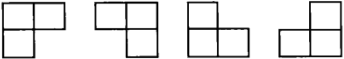
\includegraphics{lplate.png}\\
\figcaption{4种L型牌}\label{fig:lplate}
\end{center}

\subsubsection{输入}
第一行包含一个整数T,表示有T组测试用例。

每一组测试用例占用一行,包含一个整数k。

\subsubsection{输出}
所需L型牌的总数

\subsubsection{样例输入}
\begin{Code}
3
1
2
3
\end{Code}

\subsubsection{样例输出}
\begin{Code}
1
5
21
\end{Code}

\subsubsection{分析}
本题的棋盘是$2^k \times 2^k$,很容易想到用分治法。把棋盘切成4块,则每一块都是$2^{k-1} \times 2^{k-1}$的。有黑格的那一块可以递归解决,但其他3块并没有黑格子,应该怎么办呢?可以构造出一个黑格子,如图~\ref{fig:chessboard}所示,在中心放一个L型牌,其它3块也变成了子问题。递归边界不难得出,当$k=1$时1块L型牌就够了。
\begin{center}
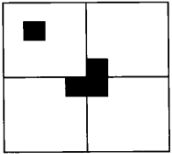
\includegraphics{chessboard.png}\\
\figcaption{棋盘覆盖问题的递归解法}\label{fig:chessboard}
\end{center}

本题只需要求总数,不需要求具体怎么摆放,因此简化很多。根据上面的思路,设$f(k)$表示棋盘是$2^k \times 2^k$时所需L型牌的总数,可得递推公式$f(k)=4f(k-1)+1$。

注意,$2^100$是一个很大的数,本题需要处理大数,见\S \ref{sec:bigintmul}节。

\subsubsection{代码}
\begin{Codex}[label=chessboard_cover.c]
#include<stdio.h>
#include<string.h>

#define MAXK 100

/* 一个数组元素表示4个十进制位,即数组是万进制的 */
#define BIGINT_MOD 10000
#define MOD_LEN 4
#define MAX_LEN (61/MOD_LEN+1)  /* 整数的最大位数, 10^x > 4^100 */

int  d[MAXK][MAX_LEN * 2];  /* d[k-1] = f(k) */

/**
 * @brief 打印大整数.
 * @param[in] x 大整数,用数组表示,低位在低地址
 * @param[in] n 数组x的长度
 * @return 无
 */
void bigint_print(const int x[], const int n) {
    int i;
    int start_output = 0;  /* 用于跳过前导0 */
    for (i = n - 1; i >= 0; --i) {
        if (start_output) {  /* 如果多余的0已经都跳过,则输出 */
            printf("%04d", x[i]);
        } else if (x[i] > 0) {
            printf("%d", x[i]);  /* 本题输出比较坑爹,最高位数字有前导0 */
            start_output = 1; /* 碰到第一个非0的值,就说明多余的0已经都跳过 */
        }
    }

    if(!start_output) printf("0");  /* 当x全为0时 */
}

/**
 * @brief 计算f(k) = 4f(k-1)+1,与大整数乘法很类似.
 * @param[in] x x
 * @param[in] y y
 * @param[out] z z=x*y+1
 * @return 无
 */
void bigint_mul_small(const int x[], const int y, int z[]) {
    int i;
    for (i = 0; i < MAX_LEN * 2; i++) z[i] = 0;

    z[0] = 1;

    for (i = 0; i < MAX_LEN; i++) z[i] += x[i] * y;
    
    for (i = 0; i < MAX_LEN * 2; i++) {  /* 统一处理进位问题 */
        if (z[i] >= BIGINT_MOD) {  /* 看是否要进位 */
            z[i+1] += z[i] / BIGINT_MOD;  /* 进位 */
            z[i] %= BIGINT_MOD;
        }
    }
}

int main() {
    int k, T;
    d[0][0] = 1;
    for (k = 2; k <= 100; k++) bigint_mul_small(d[k-2], 4, d[k-1]);

    scanf("%d", &T);
    while(T-- > 0) {
        scanf("%d", &k);
        bigint_print(d[k - 1], MAX_LEN * 2);
        printf("\n");
    }
    return 0;
}
\end{Codex}

\subsubsection{类似的题目}
与本题相同的题目:
\begindot
\item 《算法竞赛入门经典》\footnote{刘汝佳,算法竞赛入门经典,清华大学出版社,2009}第148页8.3.3节
\item NYOJ 45 棋盘覆盖, \myurl{http://acm.nyist.net/JudgeOnline/problem.php?pid=45}
\myenddot

与本题相似的题目:
\begindot
\item POJ 2495 Incomplete chess boards, \myurl{http://poj.org/problem?id=2495}
\myenddot


\section{循环赛日程表} %%%%%%%%%%%%%%%%%%%%%%%%%%%%%%

